\documentclass{sigchi}

% Use this command to override the default ACM copyright statement (e.g. for preprints). 
% Consult the conference website for the camera-ready copyright statement.


%% EXAMPLE BEGIN -- HOW TO OVERRIDE THE DEFAULT COPYRIGHT STRIP -- (July 22, 2013 - Paul Baumann)
% \toappear{Permission to make digital or hard copies of all or part of this work for personal or classroom use is 	granted without fee provided that copies are not made or distributed for profit or commercial advantage and that copies bear this notice and the full citation on the first page. Copyrights for components of this work owned by others than ACM must be honored. Abstracting with credit is permitted. To copy otherwise, or republish, to post on servers or to redistribute to lists, requires prior specific permission and/or a fee. Request permissions from permissions@acm.org. \\
% {\emph{CHI'14}}, April 26--May 1, 2014, Toronto, Canada. \\
% Copyright \copyright~2014 ACM ISBN/14/04...\$15.00. \\
% DOI string from ACM form confirmation}
%% EXAMPLE END -- HOW TO OVERRIDE THE DEFAULT COPYRIGHT STRIP -- (July 22, 2013 - Paul Baumann)


% Arabic page numbers for submission. 
% Remove this line to eliminate page numbers for the camera ready copy
% \pagenumbering{arabic}


% Load basic packages
\usepackage{balance}  % to better equalize the last page
\usepackage{graphics} % for EPS, load graphicx instead
\usepackage{times}    % comment if you want LaTeX's default font
\usepackage{url}      % llt: nicely formatted URLs
\usepackage{tabulary}

% llt: Define a global style for URLs, rather that the default one
\makeatletter
\def\url@leostyle{%
  \@ifundefined{selectfont}{\def\UrlFont{\sf}}{\def\UrlFont{\small\bf\ttfamily}}}
\makeatother
\urlstyle{leo}


% To make various LaTeX processors do the right thing with page size.
\def\pprw{8.5in}
\def\pprh{11in}
\special{papersize=\pprw,\pprh}
\setlength{\paperwidth}{\pprw}
\setlength{\paperheight}{\pprh}
\setlength{\pdfpagewidth}{\pprw}
\setlength{\pdfpageheight}{\pprh}

% Make sure hyperref comes last of your loaded packages, 
% to give it a fighting chance of not being over-written, 
% since its job is to redefine many LaTeX commands.
\usepackage[pdftex]{hyperref}
\hypersetup{
pdftitle={SIGCHI Conference Proceedings Format},
pdfauthor={LaTeX},
pdfkeywords={SIGCHI, proceedings, archival format},
bookmarksnumbered,
pdfstartview={FitH},
colorlinks,
citecolor=black,
filecolor=black,
linkcolor=black,
urlcolor=black,
breaklinks=true,
}

% create a shortcut to typeset table headings
\newcommand\tabhead[1]{\small\textbf{#1}}


% End of preamble. Here it comes the document.
\begin{document}

\title{Carbon Tax Calculator to Help Foster Informed Voting}

\numberofauthors{3}
\author{
  \alignauthor Justin Bare\\
    \affaddr{University of Washington}\\
    \affaddr{Seattle, WA, USA}\\
    \email{jbare@cs.washington.edu}\\
    \affaddr{}
}

\maketitle

\begin{abstract}
A string of Supreme Court decisions has allowed a massive influx of money into the political processes of the United States. The resulting rapid increase in the amount of biased information has made it difficult for Americans to find relevant facts that they can trust to help them decide on political issues. We have a vision of using online tools to introduce facts into the political sphere in ways that are transparent and fair, and that hold the producers of facts accountable for the information they provide. As a prototypical example, we are working on a calculator for a revenue neutral carbon tax proposal in the state of Washington. We will augment the tool with several novel features aimed at facilitating voters' understanding of the policy and its impacts. To this end we will employ a value sensitive design approach to create the features and evaluate how effective they are at supporting the values people desire from political information sources. 
\end{abstract}

\keywords{
	Value Sensitive Design; politics
}

%\category{H.5.m.}{Information Interfaces and Presentation (e.g. HCI)}{Miscellaneous}

%See: \url{http://www.acm.org/about/class/1998/}
%for more information and the full list of ACM classifiers
%and descriptors. \newline
%\textcolor{red}{Optional section to be included in your final version, 
%but strongly encouraged. On the submission page only the classifiers’ 
%letter-number combination will need to be entered.}

\section{Introduction}

Several recent United States Supreme Court decisions \cite{supremeCourt} have 
significantly weakened campaign finance laws. Corporations and wealthy individuals 
have taken advantage of these changes by massively increasing their campaign contributions. 
Spending in 2012 rose to more than one billion dollars, about three times the amount spent in 2008 
\cite{spending}. This makes it difficult for citizens to find information 
that they can trust because they are never sure who is funding advertisements or other information sources.

Our current project is one step toward countering the flood of money and misinformation. By itself this is clearly not enough, but along with other political activity, it might help tilt the balance. Our goal is to provide high-quality information for the debate around this particular initiative, as well as a model that can be replicated for providing high-quality information. We aim to create a tool that 
supports the values that people desire from their information sources - in particular the values 
of transparency, fairness, and accountability. This specific project 
deals with a calculator tool for a revenue neutral carbon tax swap policy designed by the Carbon Washington organization 
that may be voted on in the near future. However, we hope that the design process and features developed will be transferable 
to many other political issues.

The Carbon Washington revenue-neutral carbon tax proposal is composed of four main parts: 
\begin{enumerate}
\item reducing the state sales tax,
\item funding a tax rebate for low income households,
\item eliminating a business tax for manufacturers,
\item and instituting a tax on fossil fuels.
\end{enumerate}
``Revenue-neutral'' means that the total amount that the Washington state government raises 
from taxes every year will not change significantly as a result of this policy. The revenue 
reductions (1 and 3 above) and the additional spending (2) will be balanced by the new 
revenue source of the tax on fossil fuels (4).  

The calculator is meant to inform stakeholders about the estimated effects of this policy 
on their interests. For example, individuals will be able to see how the different tax changes will affect their 
household finances. But we do not want this tool to be another element of partisan misinformation campaigns. Rather we hope to design a tool that a majority of stakeholders trust to give reliable, accurate information 
that will allow them to vote on the policy knowing that they have an adequate understanding of its implications. 
To effectively incorporate the values mentioned above into our tool, we will make use of Value Sensitive Design 
techniques throughout the design process. 

\section{Conceptual Investigation}
To get a better sense of the landscape of ideas that could go into this project, 
we began with a conceptual investigation of the stakeholders and values 
implicated in the calculator. 

\subsection{Stakeholder Analysis}

We brainstormed a list of stakeholders in the project and analyzed the ways they 
could be affected by the tool. Then we synthesized values from these effects 
and determined the value tensions among the stakeholders. This work is shown in 
Tables \ref{tab:direct} and \ref{tab:indirect}. 

\begin{table*}
  \centering
  \resizebox{\textwidth}{!}{
  \begin{tabular}{|p{0.2\textwidth}|p{0.2\textwidth}|p{0.2\textwidth}|p{0.2\textwidth}|p{0.2\textwidth}|}
    \hline
    \tabhead{Direct Stakeholders} &
    \tabhead{Benefits} &
    \tabhead{Harms} &
    \tabhead{Values} &
    \tabhead{Tensions} \\
    \hline
    Environmentally conscious citizens and businesses  & Portrayal of carbon tax is positive & Portrayal of carbon tax is negative & Sustainability \newline Economic strength  & Usability for other stakeholders \newline Economic strength based on fossil fuels \\
    \hline
    Not environmentally conscious citizens and businesses  & Portrayal of carbon tax is negative & Portrayal of carbon tax is positive & Economic strength  & Usability for other stakeholders \newline Sustainability \\
    \hline
    Policy wonks  & More detailed information to analyze &  & Detail  & Usability for other stakeholders  \\
    \hline
    Journalists & Could have a popular article & Could have an unpopular article & Intrigue \newline Narrative  & Usability for other stakeholders  \\
    \hline
    All of the above & Better understanding of the policy & Deceived by the information provided & Transparency \newline Fairness \newline Accountability \newline Usability & Personal beliefs about sustainability may conflict with these values \\
    \hline
    
  \end{tabular}}
  \caption{Direct stakeholder analysis.}
  \label{tab:direct}
\end{table*}

As we can see, all direct stakeholders are generally interested in having a tool they can trust that is transparent, 
accountable, and fair. However, these values are in tension with personal beliefs about sustainability. So for example, an environmentally conscious citizen may value the calculator more if she perceives it as making more of a positive judgement about the carbon tax. Citizens are divided on the issue of sustainability depending 
on what they think about climate change. All citizens value economic strength, however 
some view sustainability as a critical piece of economic strength. Policy wonks and journalists 
have particular values that relate to their work. Because different users have different needs, 
their usability values may be in conflict. Members of marginalized groups are often in lower income 
brackets, so they would benefit from a calculator that portrays the carbon tax policy more positively, since 
it includes a rebate for low income families. Also, they may have particular usability needs (e.g. blind or low vision people). 

\begin{table*}
  \centering
  \resizebox{\textwidth}{!}{
  \begin{tabular}{|p{0.2\textwidth}|p{0.2\textwidth}|p{0.2\textwidth}|p{0.2\textwidth}|p{0.2\textwidth}|}
    \hline
    \tabhead{Indirect Stakeholders} &
    \tabhead{Benefits} &
    \tabhead{Harms} &
    \tabhead{Values} &
    \tabhead{Tensions} \\
    \hline
    Environmentally conscious politicians and organizations  & Portrayal of carbon tax is positive & Portrayal of carbon tax is negative & Sustainability \newline Economic strength  & Economic strength based on fossil fuels \\
    \hline
    Not environmentally conscious politicians and organizations  & Portrayal of carbon tax is negative & Portrayal of carbon tax is positive & Economic strength  & Sustainability \\
    \hline
    Social justice politicians and organizations  & Portrayal of policy is positive \newline Website is accessible & Portrayal of policy is negative \newline Website is not accessible & Equity  & Usability for other stakeholders \newline Economic strength \\
    \hline
    All of the above & Constituents have a better understanding of the policy & Constituents are deceived by the information provided & Transparency \newline Fairness \newline Accountability & Official positions on sustainability may conflict with these values \\
    \hline
    
  \end{tabular}}
  \caption{Indirect stakeholder analysis.}
  \label{tab:indirect}
\end{table*}

For the indirect stakeholders, the value assignments and tensions play out similarly. Many 
of the aforementioned values are still important for these stakeholders, but this is often in terms of 
how their constituents or members would be affected. 


\subsection{Researcher Stance}
To clarify our roles as researchers on this project, we also explored 
our values, the designer values, in relation to the calculator. We personally 
value sustainability and equity. We also value economic strength, but through 
sustainability with the idea that continued human endeavors depend on preventing 
severe climate change. However, we also value the explicitly supported values of this project 
in terms of fostering a healthy political system in which citizens vote confidently 
with a reasonable belief that they can trust the information they have received. Therefore, we 
are putting aside our specific personal values for this project to design a tool that 
all stakeholders will hopefully deem credible. 

\subsection{Conceptions of Key Values}
In the following sections we'll take a more in depth look at the philosophical conceptions 
of the three key values in order to get a better idea of what our tool needs to support. 

\subsubsection{Transparency}
The following two definitions offer conceptions of transparency that will be relevant to the 
work of this project. Moser offers the definition ``to open up the working procedures not immediately 
visible to those not directly involved in order to demonstrate the good working of an institution'' \cite{moser}. 
Another definition is ``the disclosure of information by an organization that enables external actors to 
monitor and assess its internal workings and performance'' \cite{compMediated}. 

Therefore, users should be able to access the internal workings of our tool in order to verify that they are in 
fact calculating the values correctly. This appears to be easy since the Javascript code for the website can be 
viewed directly in a browser. However, a key part of transparency for our purposes will be comprehensibility. Not 
all users are going to be able to understand Javascript, so we need to somehow expose the code behind the calculations 
to demonstrate proper computation in a way that is accessible to stakeholders who do not know programming.

\subsubsection{Accountability}
Two definitions of accountability are ``the sense of individual responsibility and concern for the 
public interest'' \cite{mulgan} and ``public  accountability  involves  answering,  through  various 
mechanisms  from  newspaper  reports  to  hearings,  public  concerns  about  administrative 
activity'' \cite{sinclair}. 

This will be a difficult value to design for - the first definition offers accountability as a kind of 
spiritual guide to follow to make sure anything that you do is in the public interest. The second 
definition is more practical and suggests that we design features that allow us to answer to criticisms 
from users in a public setting. 

\subsubsection{Fairness}
It was difficult to find concise useful conceptions of fairness, so here we use
impartiality instead, which is closely related, but we will outline the distinction as we see it. 

John Stuart Mill defined impartiality as ``being exclusively influenced by the considerations 
which it is supposed ought to influence the particular case in hand; and resisting the 
solicitation of any motives which prompt to conduct different from what those considerations 
would dictate'' \cite{mill}. Another possible conception is ``not that everyone receive equal 
treatment, but rather that everyone be treated as an equal'' \cite{stanford}. This second definition 
hints at what we believe to be an important part of fairness which is that all people's issues 
should be addressed. So if we present the environmental and financial perspectives on the policy, 
we also should present the jobs perspective. Even if the environmental and financial perspectives 
are presented in a perfectly impartial fashion, to be fair to people who care about jobs we should 
present the analysis of the policy's effects on jobs. Impartiality seems to require detachment from 
influencing interests, while fairness includes this as well as positive support for impartial 
information pertaining to the perspectives of all possible interests. 

To these ends we will need to make sure that we provide more and more information through 
new features in a balanced fashion - not prioritizing some information agendas 
as more legitimate than others. And of course Mill's definition restates our promise to leave 
out personal values that are not the explicitly supported values in the design. 

\subsection{Value Scenarios}
To inform the design of specific features, we explored several value scenarios 
to see what information different stakeholders may be interested in having access to. 
\subsubsection{Scenario One}
``Sarah wanted to figure out how to vote on the carbon tax issue. She used the calculator and found out she would gain money from the policy, and it sounded like a good idea, so she decided to vote yes on the ballot. But then she saw an ad on TV talking about how this policy would ruin economic growth in Washington. Because of that, she decided to vote no. After the election, she found out that this ad was funded by ExxonMobil and regretted her decision.''

This scenario was crucial in expanding our ideas about how this calculator tool fits into the larger 
political sphere. At the outset, we considered the outcome of our project to be a sort of beacon of 
virtue in the information market. However, there will be other interests actively working 
against the information we provide. We need to engage with this to provide transparency in a larger 
sense than just exposing our tool's inner workings. One idea to address this is to add a feature 
that list the all the public advertisements about the policy along with where the funding for each 
advertisement came from. 

\subsubsection{Scenario Two}
``Kate wanted to figure out how to vote on the carbon tax issue. She saw there was a calculator tool that would give her 
some quality information, so she went to check out the website. However, when she got there she felt overwhelmed by the amount 
of information available. She would hover over tooltips that told her way more than she ever wanted to know about the inner workings 
of the tool. 
And there were so many issues addressed, like the financial impacts of the policy, the environmental impacts, and 
the effect on jobs, among many others. She figured there was no way she could compute the tradeoffs among all of these, 
so she gave up and decided not to vote on this issue.''

This scenario shows a tension between transparency and information overload. This will be a difficult aspect to address. 
One way would be to keep the amount of information to a minimum, but this runs the risk of not being fair to 
various interests that would like ways to analyze the effects of the policy on specific aspects of society that they value. 
Another way to address the tension could be to provide some kind of scaffolding for users to figure out how they would trade off 
the different benefits and costs of the policy. 

\section{Technical Investigation}
This quarter we made two additions to the calculator: a version for businesses to compute the estimated 
impacts of the policy on their finances and a tooltip feature to support the value of transparency. 

\subsection{Business Calculator}
The calculator for businesses is similar to the one for households except it includes the section 
for B\&O manufacturing tax reductions instead of the rebate for low income families. Also, the 
required inputs have been adjusted to align with the kind of information that business owners 
will have about their finances. For example, we do not estimate how much sales tax a business pays 
because business owners will have this information available in their budget records. Developing 
this part of the website was a crucial step in supporting fairness because business owners are 
direct stakeholders that should be given the ability to determine how the Carbon 
Washington policy would affect them. It would be unfair to have a tool that only works for 
households. 

\subsection{``Where did this number come from?''}
The other technical investigation we performed was the design of a ``where did this number come from?'' tooltip feature, which is shown in Figure \ref{fig:tooltip}. The purpose of this feature is to support transparency, and especially the comprehensibility aspect of transparency. 
For example, users of the household calculator may be unsure of how we estimated their annual sales tax payments 
from their income. Without the tooltip feature, they could read through the Javascript code to figure this out. 
However, many users will not have adequate programming knowledge or even just adequate time for this to be a 
reasonable mode of transparency. So we added this tooltip which is accessed by hovering the pointer over a question mark icon 
next to the sales tax estimate line. Doing this causes a box to appear which shows a graph of the government data we use to perform the 
computation. It also includes a brief explanation of this graph and a link to the source document for the data. 
\begin{figure*}[t]
\centering
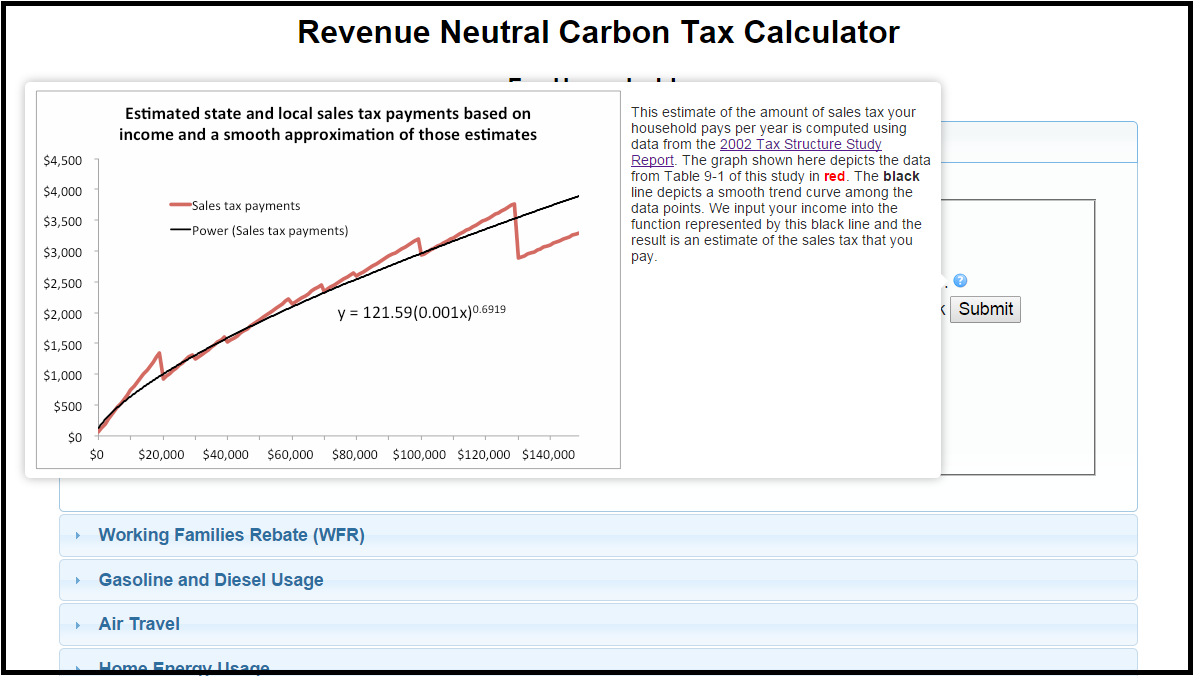
\includegraphics[width=0.9\textwidth]{toolTipDemo}
\caption{Tooltip that explains how a user's sales tax is estimated from their income in order to support the value of transparency.}
\label{fig:tooltip}
\end{figure*}


\section{Future Work}
\subsection{Future Features}
In addition to the feature ideas that came out of the value scenarios above, we would like to develop other features to serve the explicitly supported values more completely:
\begin{itemize}
\item A section showing statewide impacts of the policy in interactive graphs would be helpful 
to provide a greater understanding of the societal impact, which would be especially helpful 
for policy wonks and journalist, but also other citizens. 
\item A feature similar to public bug report forums for software would allow us to provide 
public accountability through answering any complaints that people have about the tool. 
\item Videos explaining how each section of the calculator works could provide transparency 
about the inner workings through a different medium that may be preferred by some users. 
\item A section showing estimates of how much carbon dioxide would be saved through the policy and how the policy would affect jobs would 
help to balance out the current financial focus of the tool. 
\item Visualizations of the uncertainty in the estimates of the calculator would serve transparency 
by acknowledging that these values are indeed estimates and real life effects may be different. 

\end{itemize}

\subsection{Empirical Investigation}
Once more features have been added, we will use an empirical investigation to determine how well 
the features support the values of stakeholders. 
Did users think the calculator was fair? Did they understand how the values were being calculated, 
or at least did they feel like this information was accessible if they wanted to know 
about the underlying computations? This would involve 
surveys and interviews with people who have already used the tool, as well as laboratory tests 
to obtain more detailed information on users during interactions with the tool. 

\section{Acknowledgments}

This material is based upon work supported by the National Science Foundation
Graduate Research Fellowship Program under Grant No. (NSF grant number).

% Balancing columns in a ref list is a bit of a pain because you
% either use a hack like flushend or balance, or manually insert
% a column break.  http://www.tex.ac.uk/cgi-bin/texfaq2html?label=balance
% multicols doesn't work because we're already in two-column mode,
% and flushend isn't awesome, so I choose balance.  See this
% for more info: http://cs.brown.edu/system/software/latex/doc/balance.pdf
%
% Note that in a perfect world balance wants to be in the first
% column of the last page.
%
% If balance doesn't work for you, you can remove that and
% hard-code a column break into the bbl file right before you
% submit:
%
% http://stackoverflow.com/questions/2149854/how-to-manually-equalize-columns-
% in-an-ieee-paper-if-using-bibtex
%
% Or, just remove \balance and give up on balancing the last page.
%
\balance

% REFERENCES FORMAT
% References must be the same font size as other body text.
\bibliographystyle{acm-sigchi}
\bibliography{sample}
\end{document}
